\documentclass[11pt,aspectratio=169]{beamer}
\usepackage[T1]{fontenc}
\usepackage{lmodern}
\usepackage{amsmath,amssymb,mathtools}
\usepackage{booktabs,tabularx,array}
\usepackage{pgfplots}
\pgfplotsset{compat=1.17}
\setbeamertemplate{navigation symbols}{}
\setbeamertemplate{itemize items}[circle]
\setbeamertemplate{footline}[frame number]
\setbeamerfont{framesubtitle}{size=\small}
\linespread{1.08}
\definecolor{sourcegray}{RGB}{95,95,95}
\definecolor{plotblue}{RGB}{47,74,135}
\newcommand{\source}[1]{\par\vspace{0.25em}{\tiny\color{sourcegray}Source: #1}}
\newcommand{\interpretation}[1]{\vfill{\small #1}}
\newcolumntype{Y}{>{\raggedright\arraybackslash}X}
\title{Fertility and Housing Tenure Choice}
\author{Tommaso De Santo}
\date{September 30, 2026}
\hypersetup{pdftitle={JMP progress, September 17--30, 2026},pdfauthor={Tommaso De Santo}}
% Separate adviser progress deck. Main source latex/JMP_slides/JMP_slides.tex is read-only.
% Exactly ten frames, no overlays or separate title/section/appendix pages.
% Relative source paths below are in Fertility_Spring26. See source_map.md for full paths.
\begin{document}

% 1: docs/model/situation_report_20260918.md; CALIBRATION_STATUS.md Sept23--30;
% docs/model/calibration_identification_review_20260929.md.
\begin{frame}{Fertility and Housing Tenure Choice}
\framesubtitle{JMP progress, September 17--30, 2026 \qquad Tommaso De Santo}
\textbf{Question.} How does access to family-sized housing affect births,
and which housing policies can change fertility?
\medskip
\begin{itemize}\setlength\itemsep{9pt}
  \item Mechanism tests separate mortgage access, unsecured liquidity, and space costs.
  \item Revised household preferences and accounting support a new 2007 reference.
  \item Rebuilt housing evidence and richer fertility moments sharpen the fit diagnosis.
  \item Faster stationary computation makes controlled recalibration more practical.
\end{itemize}
\interpretation{The main remaining fit problem is the number of children among young mothers.}
\source{PSID, CPS, AHS, and model experiments, September 17--30}
\end{frame}

% 2: situation_report_20260918.md, section 1. Fixed-psi early sandbox comparisons.
% Sandbox levels differ from exact September14 replay. No cross-contract loss comparison.
\begin{frame}{Mortgage access and unsecured liquidity}
\small
Early diagnostics hold the child-benefit level and other parameters fixed:
\medskip
\begin{center}
\begin{tabular}{lrrr}
\toprule
 & Baseline & No down payment & Unsecured credit \\
\midrule
Completed fertility & 1.872 & 1.866 & 1.948 \\
Mean first-birth age & 26.960 & 26.970 & 25.790 \\
Ownership, ages 30--55 (\%) & 45.9 & 55.7 & 45.0 \\
\bottomrule
\end{tabular}
\end{center}
\medskip
The unsecured-credit diagnostic allows five years of earnings.
\begin{itemize}\setlength\itemsep{5pt}
  \item Removing the down payment primarily increases homeownership.
  \item Unsecured liquidity increases births and brings them forward.
  \item Family-sized rental space limits the connection between buying and births.
\end{itemize}
\interpretation{These are comparisons within the early sandbox, before the later specification and recalibration.}
\source{Model mechanism diagnostics, September 17--19}
\end{frame}

% 3: selected_export/primary/parameters.csv; child_preferences.py;
% CALIBRATION_STATUS Sept24 dependency/entry and Sept26 estate-funded-entry decisions.
\begin{frame}{Household preferences and demographic accounting}
\small
A first-child housing-share loading replaces the hard housing floor:
\[
 \alpha(m)=\alpha_0-\Delta\alpha\,\mathbf 1\{m>0\},
 \qquad v(m)=\psi\,m^{1-\gamma},\quad v(0)=0.
\]
Here $m$ counts children at home. $\alpha(m)$ is the consumption share,
$\psi$ the direct benefit level, and $\gamma$ its curvature.
\medskip
\begin{itemize}\setlength\itemsep{6pt}
 \item Material utility retains CRRA, equivalence scales, and persistent earnings risk.
 \item Shares are compensated at a fixed rent, with no later-child loading.
 \item Dependency ends with probability $2/9$ per four-year period. Adult entry is a separate queue, split equally after 16 and 20 years.
 \item Estates fund positive entrant assets. An explicit sink absorbs the remainder.
\end{itemize}
\interpretation{Concurrent children and lifetime births are distinct calibration objects.}
\source{Model specification and author decisions, September 24--28}
\end{frame}

% 4: PSID sa_rooms_first_birth_v2/A2h/{coefficients,fit_receipt}.csv;
% sa_first_birth_outcomes_v3/A2h_{own,moved}/fit_receipt.csv.
% Plot uses raw coefficients and 1.96*SE pointwise intervals, omitted window shown hollow.
\begin{frame}{Housing around the first birth}
\small
PSID adults who were the reference person or spouse before the birth:
\begin{center}
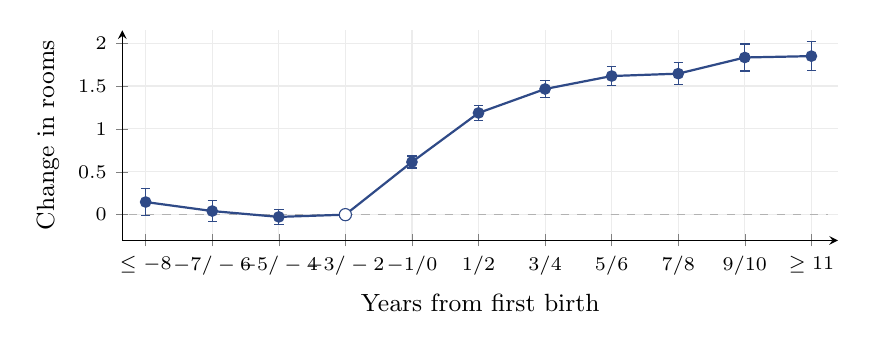
\begin{tikzpicture}
\begin{axis}[
 width=0.88\textwidth,height=4.25cm,
 xmin=-9.2,xmax=12.3,ymin=-0.3,ymax=2.15,
 xlabel={Years from first birth},ylabel={Change in rooms},
 xtick={-8.5,-6.5,-4.5,-2.5,-.5,1.5,3.5,5.5,7.5,9.5,11.5},
 xticklabels={$\leq-8$,$-7/-6$,$-5/-4$,$-3/-2$,$-1/0$,$1/2$,$3/4$,$5/6$,$7/8$,$9/10$,$\geq11$},
 tick label style={font=\scriptsize},label style={font=\small},
 axis lines=left,grid=major,grid style={gray!15},
 ytick={0,.5,1,1.5,2},
]
\addplot[gray!60,dashed] coordinates {(-9,0) (12,0)};
\addplot[plotblue,thick,mark=*,mark size=1.7pt,error bars/.cd,y dir=both,y explicit]
 table[x=x,y=y,y error=err,row sep=\\]{
 x y err\\
 -8.5 .147277343 .158189222\\
 -6.5 .042068289 .119348387\\
 -4.5 -.026169280 .087417230\\
 -2.5 0 0\\
 -.5 .613924680 .070093112\\
 1.5 1.185961330 .083049105\\
 3.5 1.465293280 .098529943\\
 5.5 1.616432695 .111654038\\
 7.5 1.644179690 .127752165\\
 9.5 1.832730146 .157289669\\
 11.5 1.848654304 .168139494\\
 };
\addplot[plotblue,only marks,mark=*,mark size=2.2pt,mark options={fill=white}] coordinates {(-2.5,0)};
\end{axis}
\end{tikzpicture}
\end{center}
\vspace{-0.8em}
At years 3--4: rooms rise by \textbf{1.465} (SE 0.050), ownership by
\textbf{26.886 pp}, and recent moving falls by \textbf{21.147 pp}.
\interpretation{Rebuilt interview dates and baseline household status resolve earlier measurement differences. Whiskers show 95\% pointwise intervals.}
\source{PSID, Sun--Abraham event study, person/year effects, IW weights, September 24}
\end{frame}

% 5: CALIBRATION_STATUS September23 national inputs, Sept24 bequest,
% Sept25 pension decision; accepted_input_reconciliation_20260926.md;
% calibration_identification_review_20260929.md.
\begin{frame}{Calibration inputs and empirical counterparts}
\small
The single housing market uses national inputs and a replacement-fertility reference.
\medskip
\begin{center}
\begin{tabular}{lll}
\toprule
Input & Value & Empirical source \\
\midrule
Mean occupied rooms & 5.729 & AHS 2007 \\
Pension / working-household earnings & 0.229 & CPS ASEC, income 2007 \\
Annual child-directed estates / wealth & 0.729\% & SCF 2007 mortality proxy \\
Annual depreciation / property tax & 1.416\% / 1.060\% & National housing inputs \\
\bottomrule
\end{tabular}
\end{center}
\medskip
\begin{itemize}\setlength\itemsep{6pt}
 \item Baseline payroll tax is 8.028\%. Equal retiree pensions balance PAYGO.
 \item The 1.465-room first-birth target has a model proxy, rather than a matched event-study estimator.
 \item Bequest and wealth targets retain recipient and income-definition gaps.
\end{itemize}
\interpretation{Fertility 2.1 normalizes the reference, rather than observed 2007 period births.}
\source{AHS 2007, CPS ASEC 2008, SCF 2007, PSID}
\end{frame}

% 6: exact full 14-row fit at resume_v1/selected_export/primary/target_fit.csv.
% Full unrounded gaps, weights, loss contributions and all31 restrictions in evidence/.
% one-child row is conditional on mothers age40--44; three validation rows daggered.
\begin{frame}{2007 stationary reference fit}
\fontsize{9}{10.7}\selectfont
{\centering\renewcommand{\arraystretch}{0.95}
\begin{tabular}{lrr}
\toprule
Moment & Target & Model \\
\midrule
Completed fertility (normalization) & 2.100 & 2.100 \\
Childlessness, ages 40--44 (\%) & 19.828 & 20.106 \\
Exactly one child among mothers, ages 40--44 (\%) & 21.366 & 20.942 \\
Mean first-birth age (years) & 25.976 & 25.933 \\
First births at age 30+ (\%)$^\dagger$ & 24.928 & 22.365 \\
Wealth / earnings & 6.927 & 6.326 \\
Annual child-directed bequest flow / wealth (\%) & 0.729 & 0.706 \\
Older wealth/income p90/p50$^\dagger$ & 3.516 & 3.069 \\
Mean occupied rooms & 5.729 & 5.848 \\
Ownership, ages 30--55 (\%) & 67.626 & 65.482 \\
First-birth rooms difference & 1.465 & 1.622 \\
Family rooms difference$^\dagger$ & 0.385 & 0.353 \\
Recent-parent ownership difference (pp) & 12.761 & 11.955 \\
\textbf{Children per woman at age 25, capped at three} & \textbf{0.810} & \textbf{0.535} \\
\bottomrule
\end{tabular}
\par}
\vspace{0.4em}
\footnotesize $^\dagger$Untargeted validation. Ten scored moments and a separate fertility normalization.
\source{CPS, NCHS, PSID, AHS, SCF, and September 28 verified model export}
\end{frame}

% 7: two_stream_overnight_v1/comparison_v1/age25_decomposition_inputs.csv;
% morning_readout_v1/RESULTS.md; calibration_identification_review_20260929.md.
\begin{frame}{Young mothers and the fertility intensive margin}
\small
Two unadopted experimental calibrations, with completed fertility normalized to 2.1:
\medskip
\begin{center}
\begin{tabular}{lrrr}
\toprule
Age-25 moment & Data & One birth per period & Two-birth option \\
\midrule
Children per woman, capped at three & 0.810 & 0.530 & 0.606 \\
Mothers (\%) & 45.725 & 44.782 & 43.773 \\
Children per mother, capped at three & 1.770 & 1.185 & 1.385 \\
\bottomrule
\end{tabular}
\end{center}
\medskip
\begin{itemize}\setlength\itemsep{7pt}
 \item The motherhood share is close. Additional births among young mothers drive the miss.
 \item The two-birth option closes 27.1\% of the early-count gap, while other fits deteriorate.
 \item Child-benefit curvature dominates a weak local parameter direction. A selected-point robustness check remains open.
\end{itemize}
\interpretation{The extra birth opportunity also adds an independent taste draw. The comparison does not isolate birth spacing alone.}
\source{CPS June 2004/2006 and model experiments, September 28--29}
\end{frame}

% 8: fixed_reference_economics_20260928/elasticity_v1/recovery_v1/collected_v1/elasticities.csv.
% Completed18815133. Fixed preferences incl b/psi, fixed entry and inherited impact weights.
% Prescribed house price + mapped rent, not GE, fixed physical stock or transition.
\begin{frame}{House prices, credit, and births}
\small
Local elasticities from prescribed house-price and rent changes of $\pm1\%$:
\medskip
\begin{center}
\begin{tabular}{lrr}
\toprule
Outcome & Reference credit & Lifetime repayment only \\
\midrule
Immediate total births & $-0.437$ & $-0.469$ \\
Immediate first births & $-0.880$ & $-0.906$ \\
Immediate second births & $-0.114$ & $-0.116$ \\
Completed fertility, recomputed cohort & $-0.536$ & $-0.555$ \\
\bottomrule
\end{tabular}
\end{center}
\medskip
First births account for 87.57\% of the immediate decline under reference credit.
\begin{itemize}\setlength\itemsep{6pt}
 \item Relaxing borrowing limits raises fertility levels at the common reference price.
 \item It leaves the local price response at least as strong in this comparison.
\end{itemize}
\interpretation{Preferences and entry stay fixed. These are prescribed-price responses, with lifetime solvency, rather than cleared equilibria or transition estimates.}
\source{Fixed-reference price and credit experiments, September 29}
\end{frame}

% 9: publication_refactor_20260929/REPORT.md; small_credit_replication_v1/README.md;
% grid_resolution_v1/credit053_v2/runner/README.md and supplemental_discrepancies.json.
\begin{frame}{Stationary computation and grid resolution}
\small
Matched comparisons preserve each experiment's economics and acceptance checks:
\medskip
\begin{center}
\begin{tabular}{lrrl}
\toprule
Comparison & Original & Revised & Result \\
\midrule
Saving routine, same $160\times15$ grid & 549 s & 417 s & 24.04\% less time \\
Grid, $160\times15$ versus $120\times9$ & 469 s & 187 s & 60.04\% less time \\
\bottomrule
\end{tabular}
\end{center}
\medskip
\begin{itemize}\setlength\itemsep{6pt}
 \item The saving optimization reproduces policies, full moment tables, and plots exactly.
 \item Grid diagnostic $D=0.53$: ownership changes by 0.201 pp and prices by 0.076\%.
 \item Ownership gaps above 5 pp cover 3.152\% of mass in the interpolated comparison.
\end{itemize}
\interpretation{Local thresholds and transitions still require validation. The grid comparison also approximates the joint wealth--income entry distribution.}
\source{Matched stationary comparisons, September 30}
\end{frame}

% 10: CALIBRATION_STATUS first section, owner thread01a0f334 last checked20:54:57UTC;
% entry_ratio_comparison_v1/README.md. Historicalfit launch_v3 failed,18820811 cancelled per author.
% D=.25 next pilot is distinct from completed D=.53 diagnostic; common interest2% annual.
\begin{frame}{Entry wealth, credit, and the next calibration}
\small
Full repayment on sale into renting, renter limit $b'\ge-D$, and a 2\% annual real rate:
\medskip
\begin{tabularx}{\textwidth}{Yr}
\toprule
Authorized one-hour exploratory arm & $D$ \\
\midrule
Empirical wealth/earnings ratios, independent of income & 0.25 \\
Zero entrant wealth & 0 \\
Nonnegative ratio nodes, rescaled to preserve the mean & 0 \\
\bottomrule
\end{tabularx}
\medskip
\begin{itemize}\setlength\itemsep{4pt}
 \item Five-ratio diagnostic at $D=0.53$: prices $+0.089\%$, ownership $-0.017$ pp, with parameters fixed.
 \item Birth-renewal price clearing makes supply scale a population shifter. The new search fixes supply scale and child benefit.
 \item Historical-shock fits yielded no estimates. The pension diagnostic was cancelled.
\end{itemize}
\interpretation{Discussion: credit/entry, curvature restrictions, and matched empirical moments. Pilots had no recorded submission at September 30, 20:55 UTC.}
\source{Author decisions and verified stationary evidence, September 29--30}
\end{frame}

\end{document}
